\makeheading{理论计算机科学中最令人迷惑的谜题之一被解开}

\vskip10pt


\noindent\fcolorbox{color1}{white}{%
\parbox{\textwidth-2\fboxsep-2\fboxrule}{\centering%
\colorbox{color2!4}{%
\parbox{\textwidth-4\fboxsep-2\fboxrule}{%

\noindent\qiangdiao{导读}

\sffamily
\ \ \ \ \ \ “自敏感度猜想提出以来,它便是所有组合学和理论计算机科学中最令人沮丧和尴尬的开放性问题之一. ”德克萨斯大学奥斯汀分校的理论计算机学家斯科特·阿伦森(Scott Aaronson)在一篇博客中写道. 阿伦森提到的猜想是一个与计算机电路的基本构件结构有关的猜想,近30年以来,许多人都试图攻克这一难题,写出了一篇又一篇长而复杂的论文,但结果都以失败告终. 然而,在一篇于本月初发表在\textrm{arXiv}上的论文中,年轻的数学家黄皓以令人惊叹的简洁方法解决了这一猜想. 

\ \ \ \ \ \  这个猜想与布尔函数有关,布尔函数是一系列将一串输入位(0和1)转换成一个独个的输出位的规则. 比如它的规则可以是,当输入字符串中的比特位全部为1时,那么输出为1,其他情况则输出为0;又比如它可以是,当输入字符串中含有1的个数为偶数时,那么输出为0,否则输出为1. 试想你正在填写一份银行贷款的申请表,你需要填写一系列“是/否”问题,银行会根据你填写的答案进行评判,然后决定你是否有资格申请贷款. 这个过程就是一个布尔函数,你的每一道“是/否”问题的答案都是一个输入位,银行的最终决定是输出位. 


}}}}

\begin{multicols}{2}

为了度量布尔函数的\qiangdiao{复杂性},计算机科学家已发展出许多不同的度量方法,每一种都针对的是“输入字符串中的信息会如何决定输出位”这一问题的不同方面. 例如布尔函数的\qiangdiao{“敏感度”}所描述的就是当一个单个的输入位被改变时,输出位因此而改变的可能性. 我们可以用上面的银行贷款例子来作进一步解释. 假如你的申请没有通过,于是你想,要是你修改某个问题的答案,是否就可以改变结果?比如在关于收入的问题上,你谎称自己年薪百万,而实际上却并没有,会不会就可以通过贷款申请?如果修改这个问题的答案真的能反转结果,那么计算机科学家会说,布尔函数对这个特定位的值是“敏感的”. 再比如说在这张长长的申请表中有7个关键的问题,如果你对这7个问题的任何一个撒谎都能反转结果,那么对于你的贷款概况而言,布尔函数的敏感度为7. 

To measure the \qiangdiao{complexity} of Boolean functions, computer scientists have developed a number of different measures, each for different aspects of how information in an input string determines the output bit. For example, the \qiangdiao{"sensitivity"} of a Boolean function describes the probability that the output bit will change when a single input bit is changed. We can use the bank loan example above to explain it further. If your application is rejected, then you think, if you change the answer to a question, can you change the result?For example, on the issue of income, you lie about your annual salary of one million, but in fact did not, can be through loan application?If changing the answer to this question really reverses the result, then a computer scientist would say that a Boolean function is "sensitive" to the value of that particular bit. If you lie about any of the seven key questions in this long application form that could reverse the result, then the sensitivity of the Boolean function is 7 for your loan profile. 

敏感度只是测量布尔函数的复杂性的其中一个度量,每种度量都为审视布尔函数的结构提供了一个独特的视角. 然而计算机科学家发现,几乎所有这些度量都符合一个统一的框架,也就是说其中的任何一个度量的值都可被用来大致衡量其他度量的值,而敏感度似乎是唯一的例外. 1992年,希伯来大学的诺姆·尼桑 (Noam Nisan)和罗格斯大学的马里奥·塞格迪(Mario Szegedy)推测,敏感度也是符合这一框架的. 但这么多年来,一直没有人能证明这一点,这个猜想成为了布尔函数研究中最突出的待解问题. 现在,埃默里大学的数学家黄皓利用立方体上的点的组合学,用仅仅两页纸的篇幅,巧妙地完成了论证. 他证明了敏感度猜想!

Sensitivity is just one measure of the complexity of Boolean functions, each of which provides a unique perspective on the structure of Boolean functions. However, computer scientists have found that almost all of these measures follow a uniform framework, meaning that the values of any one of these measures can be used to roughly measure the values of the others, with sensitivity appearing to be the only exception. In 1992 Noam Nisan of Hebrew university and Mario Szegedy of rutgers university speculated that sensitivity also fits this framework. But over the years, no one has been able to prove this, and this conjecture has become the most prominent outstanding problem in the study of Boolean functions. Now, Hao Huang, a mathematician at emory university, has cleverly demonstrated this in just two pages, using the combinatorial science of points on cubes. He proved the sensitivity conjecture!

1992年,克雷格·戈茨曼(Craig Gotsman)和纳蒂·利尼亚尔(Nati Linial)就发现,可以将敏感度猜想的证明归结为解答关于不同维度下的立方体的简单问题. 有一种方法能将含有$n$个0和1的字符串转换到$n$维立方体上的点上,那就是直接用$n$个字符位作为点的坐标. 例如你有4个2位的字符串——\texttt{00、01、10}和\texttt{11},就可以分别对应于二维平面上的一个正方形的四个角——(0,0)、(0,1)、(1,0)和(1,1);再比如你有8个3位的字符串,就可以对应于一个三维立方体的8个角,更高维度也可依次类推. 

In 1992 Craig Gotsman and Nati Linial discovered that the proof of sensitivity conjecture can be reduced to simple questions about cubes in different dimensions. One way to convert a string containing $n$ zeros and ones to a point on an $n$-dimensional cube is to use $n$ character bits as the coordinates of the points. For example, if you have four two-bit strings -- \texttt{00、01、10} and \texttt{11} -- that correspond to the four corners of a square in a two-dimensional plane -- (0,0), (0,1), (1,0), and (1,1);For example, if you have eight 3-bit strings, that corresponds to the eight corners of a three-dimensional cube, and so on. 

\begin{figure}[H]
        \centering
      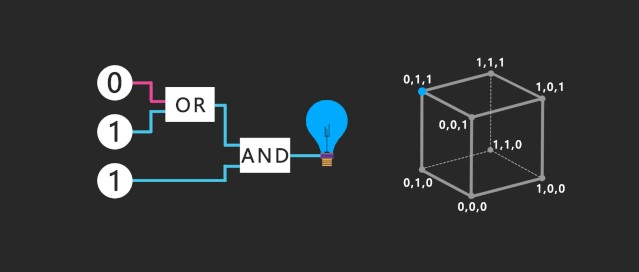
\includegraphics[width=\linewidth]{IMG/201908/1.jpg}
        \caption{ \textit{举例说明如何将$n$个输入位表示成一个$n$维立方体的坐标:如果电路输出为$1$,则灯泡亮蓝光;如果电路输出为$0$,则灯泡亮红光. }}
    \end{figure}
    
    而布尔函数可以被视作为用两种不同颜色(例如红色表示0,蓝色表示1)来对这些角进行着色的规则. 如果将一个立方体超过一半的的角着上红色,那么是否总有一些红点会与许多其他的红点相连?如果这个集合中所包含的角的个数恰好是那个立方体的一半,那么就可能没有一个角是相连的. 就比如在三维立方体的8个角中,(0,0,0)、(1,1,0)、(1,0,1)和(0,1,1)这四个点都位于对角线上. 但是,只要立方体中超过一半的点被着上了红色,那么这些红点之间就必然有一些是相连的. 问题是:这些连接是如何分布的?至少会有一个是高度相连的点吗?
    
    Boolean functions can be seen as a rule for coloring these angles in two different colors, such as red for 0 and blue for 1. If you paint more than half the corners of a cube red, will there always be some red dots connected to many other red dots?If the set contains exactly half as many angles as the cube, then none of the angles are connected. For example, in the eight corners of a three-dimensional cube, the four points (0,0,0), (1,1,0), (1,1,1), and (0,1,1) are located on the diagonal. However, as long as more than half of the points in the cube are red, some of these red points must be connected. The question is: how are these connections distributed?Is there at least one highly connected point?
    
    \begin{figure}[H]
        \centering
      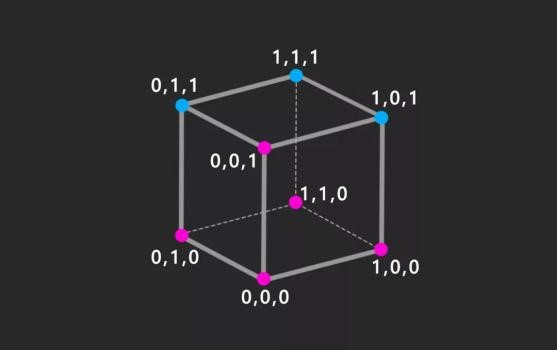
\includegraphics[width=\linewidth]{IMG/201908/2.jpg}
      \caption{\textit{立方体中有一半以上的点被着上了红色. }}
    \end{figure}
    
    黄皓决定用\qiangdiao{矩阵}来追踪哪些点是相连的,他想到了用一种已有200年历史的数学方法——\qiangdiao{柯西交错定理}(\textit{Cauchy interlace theorem}),这种方法能将矩阵的\qiangdiao{特征值}与子矩阵的特征值联系起来. 上个月他突然意识到,他只要改变矩阵中的一些数字的符号,就可以完整地将这种方法一直推演到最终结果. 通过这种方法,他成功地证明了在一个$n$维立方体中,任何超过一半的点的集合,都会有某个点至少与其他$\sqrt{n}$个点相连接——从这个结果可以立即得出敏感度猜想. 
    
    Mr. Huang decided to use \qiangdiao{matrices} to track which points are linked, and he came up with the idea of using a 200-year-old mathematical method, the \qiangdiao{Cauchy interlace theorem}, to associate \qiangdiao{eigenvalues} of matrices with those of submatrices. It occurred to him last month that by changing the sign of a few Numbers in a matrix, he could completely deduce the method all the way to the end result. In this way, he succeeded in proving that any set of more than half the points in an $n$-dimensional cube would have a point connected to at least $\sqrt{n}$ other points -- a result that immediately led to a sensitivity conjecture. 
    
    人们或许会以为,证明这样一个已经存在了30年难题,它的论证过程一定非常冗长,而且肯定极度晦涩难懂. 有的同行甚至在读之前就做好了读完之后发现自己什么都没看懂的准备. 然而,黄皓的证明却异常简明,许多研究人员一看就全明白了. 可以说,这一结果用来证明敏感度猜想绰绰有余,它所蕴含的能力或许能让我们对复杂性度量产生新的见解,是我们在未来解答布尔函数分析中的其他问题的一个强有力工具. 而且最重要的是,黄皓的研究结果消除了人们一直以来的一个担忧,那就是在复杂性度量的世界中,敏感度是否是某种奇怪的异常值. 想必有了这个结果后,许多计算机科学家都能睡得更安稳了. 
    
    One would think that the process of proving such a 30-year-old puzzle would be lengthy and, of course, extremely obscure. Some peers are prepared even before they read the book and then realize they don't understand anything. However, Huang's proof is so concise that many researchers understand it all at once. Arguably, this result is more than enough to prove the sensitivity conjecture, and its potential to shed new light on complexity metrics is a powerful tool for solving other problems in Boolean analysis in the future. And most importantly, Huang's results dispelled a long-standing concern about whether sensitivity was some strange outlier in the world of complexity measurement. Presumably, with this result, many computer  scientists will sleep better. 
\end{multicols}
\noindent \qiangdiao{参考链接}

\noindent\url{[1]https://www. quantamagazine. org/mathematician-solves-computer-science-conjecture-in-two-pages-20190725/}
\vskip-1em\ADxinhangdao\vskip2em
\begin{multicols}{2}

\noindent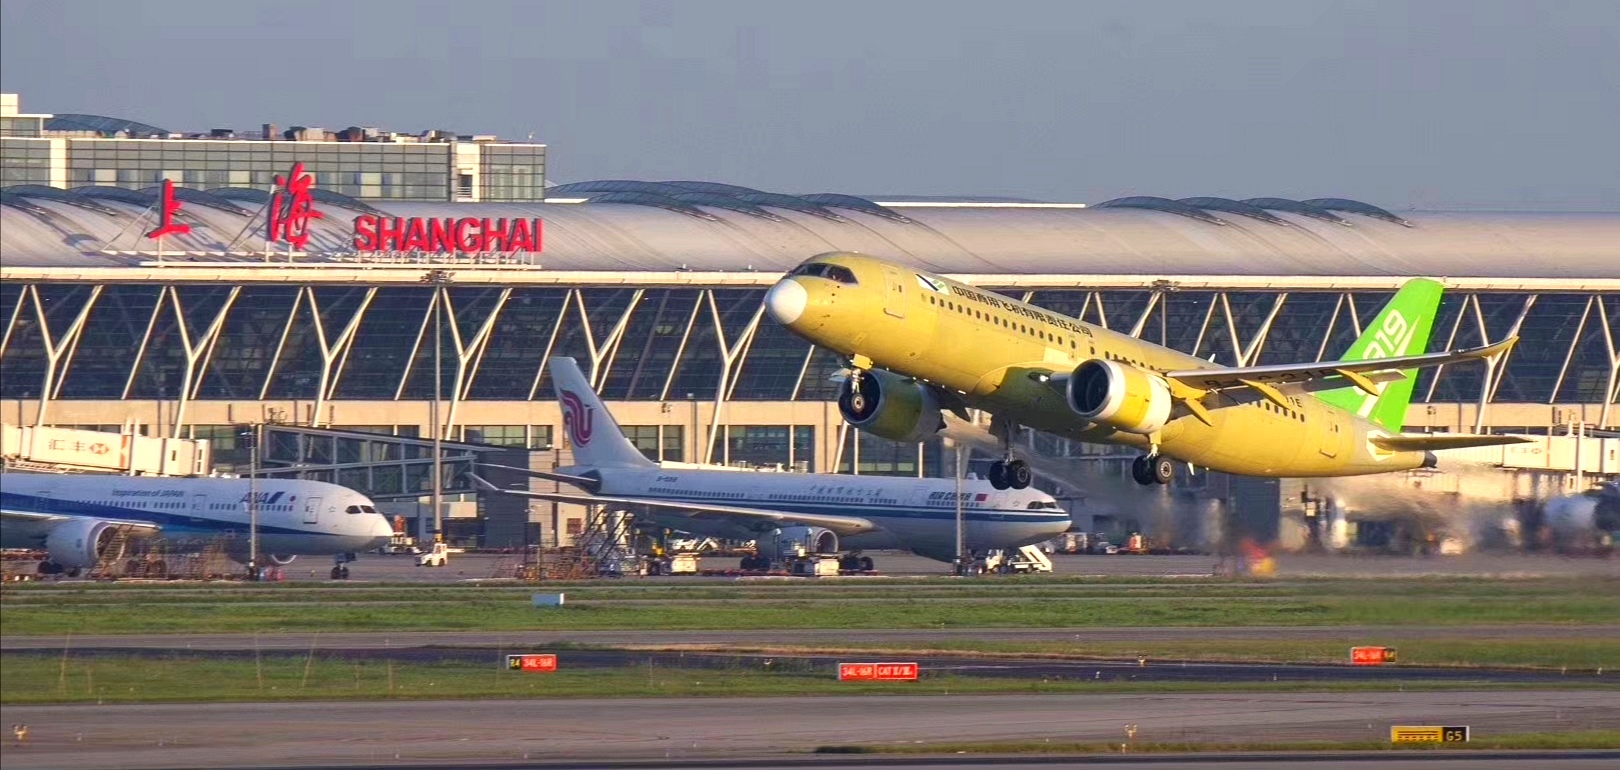
\includegraphics[width=\linewidth]{IMG/201908/7.jpg}

2019年8月1日上午,C919大型客机的第四架原型机(\textit{生产序列号}:\texttt{10104}\textit{, 注册号}:\texttt{B-001E})于5时32分在上海浦东国际机场\texttt{16L}跑道首飞,进行了1小时25分钟的飞行试验后降落. \hfill \textbf{图\copyright 冰辰海}

\noindent\fcolorbox{color1}{color2!4}{%
\parbox{\linewidth-2\fboxsep-2\fboxrule}{
  根据计划,C919将至少安排\ \qiangdiao{6架试飞飞机},针对不同科目进行验证飞行,在\texttt{104}架机之后,\texttt{105、106}架机也将在今年下半年投飞. 六架原型机各自在\qiangdiao{山东东营和西安阎良}承担不同的试飞任务,投飞之后,C919大型客机研制将进入\qiangdiao{密集试飞阶段}:


\noindent \ • \texttt{101}架机开展飞机性能,颤振、失速等试飞

\noindent \ • \texttt{102}架机验证发动机、电源、燃油等系统

\noindent \ • \texttt{103}架机验证操纵、强度、颤振、载荷、失速等

\noindent \ • \texttt{104}架机验证飞机航电,进行自然结冰试验

\noindent \ • \texttt{105}架机验证飞机的防火、环控和电源等系统

\noindent \ • \texttt{106}架机开展客舱、照明和外部噪声等试飞}}
\end{multicols}

\ADhairui

\newpage
\makeheading{生活中的科学·上期答案}

\begin{multicols}{2}

\noindent\qiangdiao{A1.}日常生活中常见的绳子打结现象是:从口袋/书包里面取出来的耳机线缠绕在一起了. 这个看起来简单的现象背后有很多科学可以细说. 由此发展的“扭结理论”是拓扑学中的一个代表研究问题,从其他的角度比如熵最大原理,统计物理理论,计算机模拟等都可以解释这一问题. 

我们用一种比较直观的过程的方法来解释整个线缠绕的过程. 如图所示,长的绳子在一个有限的容器内,为适应环境,必须以一种卷曲的姿态待在容器里,这代表,绳子的一端会与其他部分平行排放,随着容器的晃动,绳子的末端有充分的机会上下翻滚并与其他部分缠绕在一起,从而形成不同的绳结. 

明显地,形成绳结必不可少的两个因素是绳的柔性以及外界施加的微扰,具有柔性的绳在外界微扰作用下会形成绳结. 考虑到以上绳结形成的原理,可以通过限制容器的大小,外加线膜使线坚硬不易变形,合理的线缠绕保存方式等防止线的缠绕. 当然,如何合理绕线也是编织的一门手艺. 

形成的绳结是否容易打开,与绳结的具体缠绕方式有很大的关系,怎么对绳结进行分类,怎么逆向解绳,绳结在物理学或生活中有哪些应用,对这些问题感兴趣的筒子可以来物理所学习哦,当然有兴趣自学的同学可以自行搜索扭结理论(\textit{Knot theory})或辫群(\textit{Braid group}). 

 \begin{figure}[H]
        \centering
      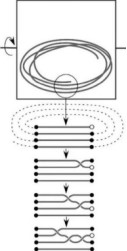
\includegraphics[angle=90,width=0.7\linewidth]{IMG/201908/3.jpg}
    \end{figure}
    
    \noindent\rule{\linewidth}{1pt}
    
    \noindent\qiangdiao{A2.}不考虑溅射的问题的话,时间是一样的. 
    
    在理想的条件下,考虑一个盆$A$在水龙头边上,另一个盆$B$在水龙头底下五米的距离,在0 s的时候开始出水(\textit{假设初始速度为}0 m/s),0 s时第一滴水以速度0 m/s的速度滴落到盆$A$,同等条件下,第一滴水需要走5 m,根据加速($g$=10 m/s$^2$)的计算,需要走1 s到达盆$B$,此时其速度为10 m/s. 假设60 s之后,盆$A$接满了水,拿走,总共用时60 s,61 s之后,盆$B$接满了水,拿走,总共用时60 s(61 s - 1 s),因此,无论是无论远近,接水时水装满盆的时间是一样的. 
    
    \noindent\qiangdiao{A3.}金属其实是没味道的. 人闻到气味,首先需要气味分子进入到鼻腔,但是金属(\textit{除了汞})在常温下是固体,和气体、液体相比,金属原子难以脱离金属表面进入鼻腔,因此直接闻金属是闻不到气味的. 那为什么金属又有气味呢?比如说铜臭味. 这其实不是金属本身的气味,是你自己的味道. 当人的皮肤和铁接触时,汗液会将单质铁氧化成二价铁,而二价铁会将皮肤上的脂质过氧化物还原成一种羰基化合物——1-辛烯-3-酮(1-octen-3-one,\begin{tabular}{c}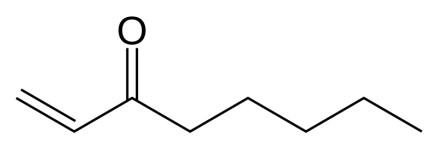
\includegraphics[width=6em]{IMG/201908/4.jpg}\end{tabular}
),这种物质就是我们平时闻到金属味的来源. 
    
    1-辛烯-3-酮广泛存在于蘑菇中,所以也有人说金属闻起来有一股蘑菇味. 血液闻起来也有金属味,这是因为血液中已经含有二价铁,可以直接将脂质过氧化物还原. 除了铁,铜也会发生类似的反应,但是氧化铝、镁、镍和人手摩擦就几乎不会有这种羰基化合物产生. 铁合金和铜合金是生活中最常见的两种金属材料,所以经常能闻到“金属味”也不奇怪了. 
    
    \noindent\rule{\linewidth}{1pt}
    
    \noindent\qiangdiao{A4.}虹吸现象是在管内液体重力与大气压的共同作用下,由于两液面间存在高度差造成的现象. 
    
     \begin{figure}[H]
        \centering
      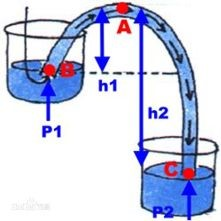
\includegraphics[width=0.4\linewidth]{IMG/201908/5.jpg}
    \end{figure}
    
    因为$h_1 < h_2$,所以根据帕斯卡定律$P=\rho gh$,左管中的液体压强$\rho gh_1$小于右管的液体压强$\rho gh_2$(\textit{压强方向向下}). 另外,在$B$点跟$C$点分别有大气压的作用(\textit{方向朝上}),可以认为两者的大气压相等即$P_1 = P_2 = P$. $B$点压强$P_B = P - \rho gh_1$,$C$点压强$P_C = P - \rho gh_2$,所以在$A$左端的压强就大于$A$右端的的压强,在大气压和液体压强的共同作用下,水朝液面低处移动,液面高度差越大流速越快. 
    
    但当$\rho gh_1\ge P$,虹吸现象就会消失. 此时管子中的水就会以$A$点为界线,左端往左流,右端往右流,中间形成一段真空层. 对水来说,这个临界的高度值为10.3米,所以生活中一般观察不到这种情况. 前面提到必须需要先用嘴吸一下,这是因为如果不用嘴吸一下管子两端的压强就是平衡的,不会自动向另一个烧杯流去. 

\end{multicols}


\makeheading{再见,“嗡嗡”}
\begin{multicols}{2}
\newcommand{\wPip }{\textit{w}PiP}
在中国的两个试验点,研究人员采用了一种对付白纹伊蚊的新方法,将它们几乎尽数消灭. 这个物种入侵性很强,而且会传播致病的病毒. 

依靠蚊子传播的病毒,包括登革热、屈公病和寨卡病毒,都是对公共卫生防疫很大的威胁. \qiangdiao{由于大部分蚊媒病毒都没有疫苗或特效药,病媒控制——遏制传播病毒的蚊虫种群——依然是减少疾病爆发的主要手段. }白纹伊蚊(\textit{也叫亚洲虎蚊,Aedes albopictus})近年来迅速散布到了更多地域,在人口密集的城市环境中也逐渐流行起来,而且它们对传统病媒控制手段的抵抗力很强. 在《自然》发表的文章中,郑小英等介绍了一种新的方案,几乎将白纹伊蚊在两个野外试验站消灭殆尽,这对未来控制白纹伊蚊和其它载病蚊类具有一定的提振作用. 

过去二十年间,涌现出了各种各样减少蚊媒病毒和其它致病微生物传播的新方案. 这些方案的目标或者是控制蚊子种群数量(\textit{称为种群抑制}),或者是通过在自然种群中扩散改造的基因或病菌感染使野生蚊子无法传播传染病(\textit{称为种群置换}). 

沃尔巴克氏体属(\textit{Wolbachia})细菌寄生在昆虫宿主的细胞内,会从母体传递到下一代,影响宿主的繁殖过程,这使得它们能同时实现种群抑制和种群置换. 举例来说,\qiangdiao{当感染某种沃尔巴克氏体的雄性伊蚊和未被感染的雌蚊交配,雌蚊将无法产下有活性的卵(\textit{图3a}). 另外,释放一些同时感染了会降低伊蚊病毒传播能力的沃尔巴克氏体的雄蚊和雌蚊,能够造成该菌株在整个种群中扩散(\textit{图3b}). }事实上,依靠沃尔巴克氏体对白纹伊蚊的近亲埃及伊蚊(\textit{Aedes aegypti})进行种群置换的田野试验正在五个国家进行. 除此之外,以前也有一些依靠沃尔巴克氏体对其它蚊类进行种群抑制的试验获得了成功. 

\begin{figure}[H]
    \centering
    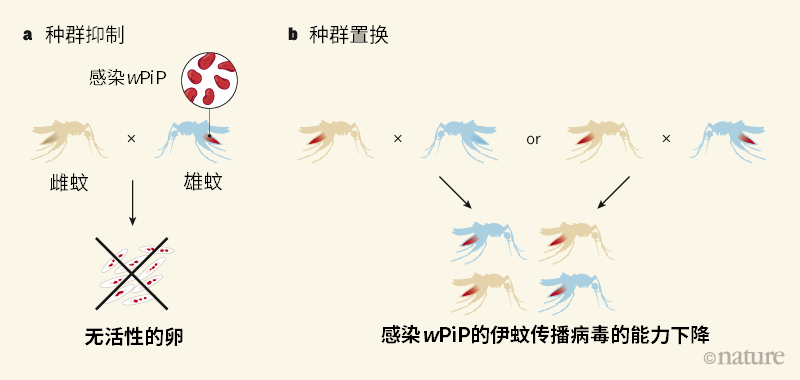
\includegraphics[width=\linewidth]{IMG/201908/6.png}
    \caption{\textit{用沃尔巴克氏体细菌来控制传播疾病的伊蚊种群}}
\end{figure}

一种控制方法叫作种群抑制,即释放被一种沃尔巴克氏体感染的雄蚊,它们无法和未感染同一菌种的雌蚊产生有生育能力的后代. 郑小英等人研究的一个目标就是用这种方法抑制白纹伊蚊的种群数量,他们释放了带有沃尔巴克氏体的\wPip 菌株的雄性白纹伊蚊,这个菌株来自于另一种蚊子尖音库蚊(\textit{Culex pipiens}). 

被特定沃尔巴克氏体菌株感染的雌蚊能够产生有活性的卵,不管与之交配的雄蚊有没有被同一菌株感染. 于是,如果感染了\wPip 菌株的雌蚊被意外释放,野生雌蚊比\wPip 雌蚊能产生后代的数量少,\wPip 菌株的感染范围会迅速在种群中扩大,实现种群置换. 但是,郑小英等人的研究表明,感染\wPip 的伊蚊比野生蚊携带致病病毒的几率更小. 因而,种群置换也能够减少病毒的传播. 

白纹伊蚊的入侵性极强,过去40年里,它们已经从原住地亚洲飞速扩散到了除南极洲之外的所有大洲. \qiangdiao{这种伊蚊很难控制,部分原因是它们的幼虫能在形形色色的人造场所中发育,很难用杀虫剂彻底杀灭,}而且它们的卵有防水性,能在休眠状态下存活很长时间. 

郑小英和同事们的计划是释放被某种沃尔巴克氏体感染的雄性白纹伊蚊,以此抑制居民区中稳定存活的伊蚊种群,试验点在中国广州市一条河中的两个小岛上. 野生的白纹伊蚊种群中有两种不会阻断病毒传播的沃尔巴克氏体感染. 研究者们于是用第三种沃尔巴克氏体感染了白纹伊蚊,\qiangdiao{这个菌株叫做\wPip ,来自于另一种蚊子尖音库蚊(\textit{Culex pipiens}),}由此在实验室中培育的一群伊蚊被他们命名为“HC群”. 当HC群的雄性白纹伊蚊和野生双菌株感染的雌蚊交配,产生的所有胚胎均会死亡,如同预计的一样,因为雌蚊没有被相同的\wPip 菌株感染(\textit{图3a}). 然而,胚胎死亡的现象在感染了\wPip 的雄蚊和同样感染\wPip 的雌蚊交配后不会出现(\textit{图3b}). 因而,这些研究者的方法中有一个风险,如果在释放的\wPip 雄蚊中混入了\wPip 雌蚊,它们就会将\wPip 感染迅速传播到整个野生种群,从而破坏靠释放\wPip 雄蚊来抑制种群数量的初衷. 但这个风险不是很大,因为他们同时发现HC群的雌蚊比野生雌蚊更难感染登革热和寨卡病毒. 所以,尽管最初的目的是种群抑制,如果意外释放了一些HC雌蚊,最差的情况也是实现种群置换(\textit{图3b})——对于公共卫生来说仍然是有益的. 

郑小英和同事们最大的创新之处在于他们培育HC群伊蚊的方法. 在大规模培育蚊子的设施中,雄蚊蛹和雌蚊蛹往往是根据尺寸不同来机械分离的. \qiangdiao{用这种方法得到的雄蚊中有一定的雌蚊混入率,大约是0.2-0.5\%,}因而需要采用额外一步人工检查来去除雌蚊蛹——靠它们不同的解剖结构来分辨. 但是,这种工作量极大的人工检查严重限制了能制备的伊蚊总量. 郑小英等人\qiangdiao{取消了人工检查这一步,用低剂量的放射线处理HC群蚊蛹,这会使雌蚊绝育,而对雄蚊的生育能力影响不大. }由于取消了人工检查的步骤,他们能够释放的雄蚊数量提高了十多倍. 

种群抑制方案的关键因素是释放的雄蚊和野生雄蚊的比例. 因而,郑小英等人用数学模型和笼养试验估算了释放雄蚊的最佳数目和时间. 在繁殖高峰期,繁育设施每周产出了500多万只雄蚊,换算到试验点是每周每公顷逾16万只. 在试验点和附近对照地(\textit{无}HC\textit{雄蚊释放}),郑小英等人监测了野生蚊的产卵数量与活性,以及成年蚊的数量和叮人率. 释放雄蚊的试验连续两年取到了惊人的效果. \qiangdiao{相比对照地,试验点的野生蚊活卵数两年均下降了94\%,}同时用装置捕获的野生成年雌蚊数在两个试验点分别降低了83\%和94\%(\textit{只有雌蚊会吸血}). \qiangdiao{更值得一提的是,估算的叮人率下降了96.6\%之多. }据调查,最初当地居民对释放试验的态度大多是怀疑或者漠不关心,后来他们的支持率从13\%上升到了54\%. 

郑小英和同事们的试验十分出色,他们在试验点几乎消灭了这种臭名昭著又极难控制的病媒蚊. 但是,这个方法的长期可持续性还有一些疑问. 例如,一旦释放停止,别地迁移来的伊蚊重建自然种群仍不可避免. \qiangdiao{这类种群重建或许能靠定向释放少量雄蚊或者其它传统的病媒控制手段来防治,但这些额外行动所需要的强度和成本仍然未知. }另外,仍不清楚这个方法能够扩大到多大的空间范围. 关于自动释放技术和性别分离方法的一些研究,将会大大提升选育和释放的能力. 但是,这些技术进步能否战胜财政和制度上的挑战,应用于主要城市群乃至全国来阻隔疾病传播,还是一个未知数. 

没有任何单一的病媒控制方案能完全控制病媒蚊;将多种手段整合起来可能才是最有效的. 不过,郑小英和同事们的研究成果代表一项重大进展,展现了一种新型强大工具对抗蚊媒传染病的潜力. 

\end{multicols}

\noindent\qiangdiao{参考文献}

\setlength{\parindent}{-3ex}\setlength{\leftskip}{2em}[1] Xiaoying Zheng et al. , (2019) ``Incompatible and sterile insect techniques combined eliminate Mosquitoes''. \textit{Nature}. DOI: 10.1038/s41586-019-1407-9

\vfill

\setlength{\parindent}{2em}\setlength{\leftskip}{0em}\greybox{\vskip-25pt


\makeheading{生活中的科学}

\ \ \ \ 生活中,想必不少同学都会遇到一些骨骼清奇的问题,有些甚至从表面上“压不住牛顿的棺材板”了?那让我们一起来看一看几个问题吧!

Q1. 为什么水珠都是圆的?

Q2. 为什么酒精喷灯的温度高于酒精灯?

Q3. 量子纠缠可以瞬时改变量子叠加态. 以一定规律测量一组纠缠中的量子,与其纠缠的另一组在很远的地方的量子就会有规律地改变量子叠加态,这样可以以摩斯电码的方式传递信息吗?

Q4. 光是怎么携带信息的呢?

\centering{\qiangdiao{怎么样?有灵感了吗?快将你的思考分享给《星空》编辑部!}

\qiangdiao{答案将在下期揭晓哦}

\qiangdiao{主编}\ 蒋有为\ Wechat: \texttt{Jerry13616483961}\ \qiangdiao{副主编}\ 王鸿硕\ Wechat: \texttt{harrywanghs}}

}

\ADyixuehui
